% === T02 - Lenguajes de descripción de Hardware (Verilog) ===
% David Alejandro Gonzalez Marquez
% fokerman@gmail.com
% https://github.com/fokerman/fpgaSoftcoreProgrammingCourse

\RequirePackage[2020-02-02]{latexrelease}

\documentclass[aspectratio=169]{beamer}
\usepackage{../packages}

\newcommand{\na}{\cellcolor{naranjauca}}
\newcommand{\gm}{\cellcolor{gray!50}} 

\title{\Huge Lenguajes de descripción\\ de Hardware (Verilog)}
\author{David Alejandro González Márquez}
\institute{Programación de softcores en FPGAs\\
Programa de Profesoras/es Visitantes\\
Departamento de computación\\
Universidad de Buenos Aires}


\date{}

\lstset{
  backgroundcolor=\color{gray!20},   % choose the background color; you must add \usepackage{color} or \usepackage{xcolor}; should come as last argument
  basicstyle=\footnotesize,        % the size of the fonts that are used for the code
  breakatwhitespace=false,         % sets if automatic breaks should only happen at whitespace
  breaklines=true,                 % sets automatic line breaking
  extendedchars=true,              % lets you use non-ASCII characters; for 8-bits encodings only, does not work with UTF-8
  keepspaces=true,                 % keeps spaces in text, useful for keeping indentation of code (possibly needs columns=flexible)
  language=Verilog,                 % the language of the code
  showspaces=false,                % show spaces everywhere adding particular underscores; it overrides 'showstringspaces'
  showstringspaces=false,          % underline spaces within strings only
  showtabs=false,                  % show tabs within strings adding particular underscores
  tabsize=2,	                   % sets default tabsize to 2 spaces
  frame=single	                   % adds a frame around the code // topline bottomline leftline
}

\begin{document}

\begin{frame}[plain]
    \titlepage
    \begin{textblock}{110}(25,80)
    \begin{tcolorbox}[size=small,width=\textwidth,colback={gray!30},title={}]
    \begin{center}
     \scriptsize Clase disponible en: \url{https://github.com/fokerman/fpgaSoftcoreProgrammingCourse}
    \end{center}
    \end{tcolorbox}
    \end{textblock}
\end{frame}

\begin{frame}[fragile,t]
    \frametitle{Hardware Description Lenguajes}
    \begin{block}{HDL}
    Lenguajes de programación que nos permiten \textbf{describir} el comportamiento o la estructura del hardware de sistemas digitales.
    \end{block}
    \pause
    Permiten especificar circuitos con \textbf{complejos diseños}, \textbf{simular} su comportamiento\\
    y \textbf{sintetizar} su implementación.\\
    \bigskip
    \pause
    Son lenguajes específicamente diseñados para describir hardware, \textbf{no son de propósito general}.\\
    \bigskip
    \pause
    Existen dos lenguajes bien conocidos de HDL.
    \begin{itemize}
     \item \textbf{VHDL} (Estándar ANSI/IEEE 1076-1993)\\
     \textcolor{verdeuca}{Desarrollado en 1981 por el Departamento de Defensa de los EEUU.}
     \item \textbf{Verilog} (Estándar IEEE 1364-2001)\\
     \textcolor{verdeuca}{Desarrollado en 1984 por Gateway Design Automation {\small(Now Cadence Design Systems)}.}
    \end{itemize}
\end{frame}

\begin{frame}[fragile,t]
    \frametitle{Diseño Jerárquico}
    \begin{textblock}{85}(10,12)
    \uncover<1->{
        El diseño jerárquico consiste en construir una jerarquía\\
        de módulos. \textcolor{verdeuca}{Desde niveles más bajos de abstracción a\\
        niveles más altos.}\\
        \bigskip
        % \textcolor{gray}{Por ejemplo:}\\
        % El nivel mas bajo utilizará primitivas predefinidas como compuertas.\\
        % El siguiente nivel consistirá en componentes como multiplexores, o sumadores, etc.\\
        % Con estos componentes construiremos modulos que definan funcionalidades simples.\\
        % Y usando modulos simples construiremos modulos más complejos.\\
    }
    \uncover<2->{
        Construir un diseño jerárquico nos permite:
        \begin{itemize}
        \item \textbf{Tener control} sobre el diseño y sobre las modificaciones o instanciaciones particulares.
        \item \textbf{Reducir la complejidad} del diseño, reduciendo comportamientos complejos a módulos.
        \end{itemize}
    }
    \uncover<3->{
        \bigskip
        \textcolor{verdeuca}{
        Sin embargo, un mal diseño puede generar\\
        \textbf{complejidad accidental} en la sintesis y 
        por lo tanto construir una implementación \textbf{ineficiente} o que \textbf{no respeta el comportamiento} esperado.
        }
    }
    \end{textblock}
    \begin{textblock}{50}(92,9)
    \includegraphics[scale=0.8]{img/diseno_jerarquico_top_down-layer1.pdf}
    \end{textblock}
\end{frame}

\begin{frame}[fragile,t]
    \frametitle{Estrategias de diseño}
    \begin{textblock}{85}(10,12)
    \uncover<1->{
        \textbf{\textcolor{naranjauca}{Top Down Design}}
        \begin{itemize}
        \item Definimos el \textbf{módulo principal} (\emph{Top module})
        \item Construimos los \textbf{Sub-Módulos} que permiten modelar el modulo principal.
        \item Diseñamos cada sub-módulo implementando otros módulos que \textbf{simplifican} el problema.
        \item Por último llegamos al \textbf{nivel de compuertas o celdas} (\emph{leaf cell}, tanto \emph{logic gates} o \emph{cell libraries}).
        \end{itemize}
    }
    \uncover<2->{
        \textbf{\textcolor{naranjauca}{Botton-Up Design}}
        \begin{itemize}
         \item Comenzamos construyendo módulos básicos.
         \item Hasta llegar a construir módulos más complejos.
        \end{itemize}
    }
    \end{textblock}
    \begin{textblock}{100}(10,76)
        \uncover<3->{\textcolor{verdeuca}{\textbf{Los buenos diseños suelen ser afrontados\\ con las dos estrategias.}}}
    \end{textblock}
    \begin{textblock}{50}(92,9)
    \includegraphics[scale=0.8]{img/diseno_jerarquico_top_down-layer2.pdf}
    \end{textblock}
\end{frame}

\begin{frame}[fragile,t]
\frametitle{¿Cómo se utiliza el código de descripción de hardware?}
    \textcolor{naranjauca}{\textbf{Sintetización (\texttt{hardware Syntesis})}}
    \begin{itemize}
    \item<1-> Herramientas mapean el código a librerías de \textbf{celdas de bajo nivel}.\\
    Construyen una \emph{netlist} de compuertas (gates) y cables (wires).
    \item<2-> Sobre la \emph{netlist} se resuelven los algoritmos de \textbf{\emph{placement} (ubicación)} y \textbf{\emph{routing} (ruteo)}.
    \item<3-> \textcolor{verdeuca}{El código debe ser escrito para que sea fácil de sintetizar, ya que no se puede garantizar encontrar una solución óptima, ni siquiera una solución.}
    %     Sobre esta estructura se pueden realizar optimizaciones para encontrar una solución que mejore el tiempo, la latencia, el consumo o el tamaño.
    %   - Sin embargo, esto no garantiza una solución optima.
    %     - El costo computacional de los algoritmos de placement (ubicación) y routing (ruteo) es muy alto, tanto que incluso puede llegar a 
    %       ser imposible encontrar una buena solución o una solución que funcione.
    %     - Por esto es necesario que el código de descripción de hardware este escrito de forma que sea facil de sintetizar.
    %   - Hace ya mucho tiempo que la descripción y sintesis de hardware es la forma en que se diseñan los sistemas,
    %     ya no es posible diseñar manualmente los sistemas transistor a transistor.
    \end{itemize}
    \uncover<4->{\textcolor{naranjauca}{\textbf{Simulación}}}
    \begin{itemize}
    \item<4-> Permite verificar el comportamiento del circuito \textbf{sin que sea manufacturado}.
    \item<5-> Valida el comportamiento tanto del \textbf{código escrito}, ya sea de forma \emph{structural} o \emph{behavioral}.
    \item<6-> La simulación es esencial para verificar el funcionamiento y \textbf{\emph{timming} del circuito}.
    \end{itemize}

    \begin{center}
    \uncover<7->{\textcolor{verdeuca}{
     Los HDL buscan describir \emph{hardware}, \textbf{NO se deben pensar como código ejecutable.}\\
     Para poder escribir esté código, se debe conocer que es lo que se busca construir.}}
    \end{center}
    % El codigo de descripción de hardware busca describir hardware, no se debe pensar como código que se ejecuta o que se comporta exactamente como fue escrito.
    % Se debe pensar como código que permitirá construir hardware. Por lo tanto es fundamental conocer de antemano y diseñar que es lo que se busca construir.
    % Se deben entender los bloques funcionales, su comportamiento y como deberían ser implementados, y luego se podrá escribir el código que los construya.
    % No podemos tener una versión de código escrita de forma muy ineficiente, ya que esta construirá hardware muy malo, que la herramienta no podrá optimizar, y que en algunos casos, tampoco podrá hacer funcionar.
\end{frame}

\begin{frame}[fragile,t]
    \frametitle{Definiendo módulos en \texttt{Verilog}}
    \begin{textblock}{60}(10,12)
    Un \textcolor{naranjauca}{\texttt{module}} es el bloque de construcción más básico de \texttt{Verilog}.\\
    \begin{center}
    \includegraphics[scale=0.8]{img/circuito_combinatorio_modulo-layer2.pdf}
    \end{center}
    \uncover<2->{
    Se define con:
    \begin{itemize}
    \item \textbf{Nombre}: Identificación del modulo, debe ser única.
    \item \textbf{Puertos}: Define cada una de las entradas y salidas.
    \item \textbf{Cuerpo}: Descripción de su funcionalidad.
    \end{itemize}
    }
    \end{textblock}
    \begin{textblock}{67}(80,8)
    \begin{onlyenv}<3->
    \textcolor{gray}{Ejemplo:}
\begin{lstlisting}
module example(a, b, c, s);
    input a;
    input b;
    input c;
    output s;
    ....
endmodule
\end{lstlisting}
    \end{onlyenv}
    \begin{onlyenv}<4->
    La dirección de los puertos se puede definir como parte de la declaración.
\begin{lstlisting}
module example(input a, input b,
                input c, output s);
    ....
endmodule
\end{lstlisting}
    \end{onlyenv}
    \end{textblock}
\end{frame}

\begin{frame}[fragile,t]
    \frametitle{Definición de entradas y salidas con múltiples bits}
    La sintaxis para definir múltiples bits es la siguiente:
    \begin{center}
    \verb|[start:end]|
    \end{center}
    Donde \texttt{start} corresponde al bit numerado como más significativo y \texttt{end} al bit numerado como menos significativo.
    \textcolor{verdeuca}{Tanto \texttt{start} como \texttt{end} \textbf{pueden tomar cualquier número} entero positivo, incluso pueden estar a la inversa.}
    \pause
    \vspace{0.3cm}
\begin{lstlisting}
    input [15:0] a; // --> a[15], a[14], a[13], ..., a[1], a[0]
    input [1:8]  b; // --> b[1], b[2], ..., b[6], b[8]
    input [3:2]  c; // --> c[3], c[2]
    output       d; // --> d (only one signal)
\end{lstlisting}
    \vspace{0.3cm}
    \pause
    \textcolor{verdeuca}{\textbf{Preferimos la forma \texttt{[15:0]} para definir multi-señales}},
    donde el comienzo es un entero positivo y final siempre es cero.\\
    \textcolor{gray}{Solo para arreglos de señales podemos usar la declaración a la inversa para evitar confusiones.}
\end{frame}

\begin{frame}[fragile,t]
    \frametitle{Tipos de datos}
    En \texttt{Verilog} las variables pueden ser de dos tipos:
    \begin{itemize}
     \item<2->[-] \textcolor{naranjauca}{Cable} (\emph{net data type})\\
     Representan cables que pueden conectar distintos circuitos lógicos.
     \vspace{0.2cm}
    \begin{itemize}
     \item[-] \textbf{\texttt{wire}}: Cable bidireccional, se puede usar para completar múltiples entradas y salidas.
     \item[-] \textbf{\texttt{wor}}: Se agrega una operación lógica OR entre todas las entradas al cable.
     \item[-] \textbf{\texttt{wand}}: Se agrega una operación lógica AND entre todas las entradas al cable.
%      \item[-] \textbf{\texttt{tri}}
     \item[-] \textbf{\texttt{supply0}}: Cable siempre conectado a cero lógico.
     \item[-] \textbf{\texttt{supply1}}: Cable siempre conectado a uno lógico.
    \end{itemize}
    \vspace{0.2cm}
     \item<3->[-] \textcolor{naranjauca}{Registro} (\emph{register data type})\\
     Representa una variable que guarda información. No necesariamente será sintetizado como un conjunto de flip-flops.
     \vspace{0.2cm}
    \begin{itemize}
     \item[-] \textbf{\texttt{reg}}: Declara un conjunto de bits de forma explicita como variable.
     \item[-] \textbf{\texttt{integer}}: Representa un número en complemento a 2 de como máximo 32 bits.
    \end{itemize}
    \vspace{0.2cm}
    \end{itemize}
    \uncover<4->{\small \textcolor{verdeuca}{Si no se indica la cantidad de bits en cada caso, el default es 1.}}
\end{frame}

\begin{frame}[fragile,t]
    \frametitle{Valores lógicos}
    En \texttt{Verilog} se define un conjunto de estados posibles.
    \begin{itemize}
     \setlength\itemsep{0cm}
      \item[] \textbf{\texttt{0}} \hspace{0.5cm} $\rightarrow$ \hspace{0.5cm} Valor lógico cero.
      \item[] \textbf{\texttt{1}} \hspace{0.5cm} $\rightarrow$ \hspace{0.5cm} Valor lógico uno.
      \item[] \textbf{\texttt{z}} \hspace{0.5cm} $\rightarrow$ \hspace{0.5cm} Alta impedancia (\emph{high-impedance}).
      \item[] \textbf{\texttt{z}} \hspace{0.5cm} $\rightarrow$ \hspace{0.5cm} Valor sin importancia estructuras de casos (\emph{dont-care}).
      \item[] \textbf{\texttt{x}} \hspace{0.5cm} $\rightarrow$ \hspace{0.5cm} Valor sin importancia (\emph{dont-care}).
      \item[] \textbf{\texttt{x}} \hspace{0.5cm} $\rightarrow$ \hspace{0.5cm} Valor desconocido (\emph{unknown}).
    \end{itemize}
    \textcolor{verdeuca}{\small Notar que \texttt{x} puede significar desconocido o sin importancia, ya que su significado depende del contexto.\\}
    \bigskip
    \pause
    Para asignar valores a variables en \texttt{Verilog} se utiliza la palabra reservada \textbf{\texttt{assign}}.\\
    \vspace{0.2cm}
    \textcolor{gray}{Ejemplo:}
\begin{lstlisting}
    assign x = 1;
    assign z = y + x;
\end{lstlisting}
\end{frame}

\begin{frame}[fragile]
    \frametitle{Definición de constantes}
    \normalsize \textcolor{naranjauca}{Simple decimal}\\ \small
    Número decimal signado de 32 bits como máximo.
\begin{lstlisting}
    410     // numero signado de 32 bits
    -22     // numero signado de 32 bits
\end{lstlisting}
    \pause
    \normalsize \textcolor{naranjauca}{Base format}\\ \small
    Formato \textcolor{azulC}{$S$} \verb|'| \textcolor{rojo}{$F$} \textcolor{amarillo}{$x \dots x$}, donde \textcolor{azulC}{$S$} es el tamaño en bits;
    \textcolor{rojo}{$F$} el formato: binario (\texttt{b}), decimal (\texttt{d});\\ % octal (\texttt{o}), 
    y \textcolor{amarillo}{$x \dots x$} los bits del número representado.
\begin{lstlisting}
    3'b010  // numero de 3 bits, representa el numero 2
    7'd-4   // numero de 7 bits, representa el -4 en complemento a dos
    'd-10   // numero de 32 bits, representa el -10 en complemento a dos
\end{lstlisting}
    \pause
    \normalsize \textcolor{naranjauca}{Parameters}\\ \small
    Es una constante con nombre. Puede no tener tamaño específico, este depende de su uso.\\
    Es asignado al momento de instanciar el módulo y queda fijo en tiempo de simulación o síntesis.
\begin{lstlisting}
    parameter RED = -1, BLUE = 2;
    parameter READY = 2'b00, BUSY = 2'11, INVALID = 2'01;
\end{lstlisting}
\end{frame}

\begin{frame}[fragile,t]
    \frametitle{Manipulación de bits}
    Supongamos las siguientes variables
\begin{lstlisting}
    wire [15:0] bus; wire [7:0] data; wire [7:0] addr;
\end{lstlisting}
    \bigskip
    \pause
    \textcolor{naranjauca}{\textbf{Bit slicing}}
\begin{lstlisting}
    assing data = bus[15:8]
\end{lstlisting}
    \pause
    \textcolor{naranjauca}{\textbf{Concatenación}}
\begin{lstlisting}
    assing bus = { data, addr }
    assing bus = { data[7:4], addr, data[3:0] }
    assing bus = { data[7:4], addr[7:4], data[3:0], addr[3:0] }
\end{lstlisting}
    \pause
    \textcolor{naranjauca}{\textbf{Duplicación}}
\begin{lstlisting}
    assing bus = { 4'd0, data[7], data[7], data[7], data[7], data[7:0] }
    assing bus = { 4'd0, 4{data[7]}, data[7:0] }
\end{lstlisting}
\end{frame}

\begin{frame}[fragile,t]
    \frametitle{Operadores Aritméticos y Lógicos}
    \begin{textblock}{80}(10,8)
    \begin{center}
    \begin{tabular}{C{1cm}C{5cm}C{1cm}} $\downarrow$ & Mayor Precedencia & $\downarrow$ \\ \hline \end{tabular}\\
    \vspace{0.2cm}
    \begin{tabular}{|C{0.8cm}|C{3.95cm}|} \hline \verb|~| & not \cellcolor[HTML]{C0C0C0} \\ \hline \end{tabular}\\
    \begin{tabular}{|C{0.3cm}|C{0.65cm}|} \hline \verb|*| & mul \cellcolor[HTML]{C0C0C0} \\ \hline \end{tabular}
    \begin{tabular}{|C{0.3cm}|C{0.65cm}|} \hline \verb|/| & div \cellcolor[HTML]{C0C0C0} \\ \hline \end{tabular}
    \begin{tabular}{|C{0.3cm}|C{0.65cm}|} \hline \verb|%| & mod \cellcolor[HTML]{C0C0C0} \\ \hline \end{tabular}\\
    \begin{tabular}{|C{0.6cm}|C{1.3cm}|} \hline \verb|+| & add \cellcolor[HTML]{C0C0C0} \\ \hline \end{tabular}
    \begin{tabular}{|C{0.6cm}|C{1.3cm}|} \hline \verb|-| & sub \cellcolor[HTML]{C0C0C0} \\ \hline \end{tabular}\\
    \begin{tabular}{|C{0.6cm}|C{0.6cm}|C{3.12cm}|} \hline \verb|<<| & \verb|>>| & shift lógico \cellcolor[HTML]{C0C0C0} \\ \hline \end{tabular}\\
    \begin{tabular}{|C{0.6cm}|C{0.6cm}|C{3.12cm}|} \hline \verb|<<<| & \verb|>>>| & shift aritmético \cellcolor[HTML]{C0C0C0} \\ \hline \end{tabular}\\
    \begin{tabular}{|C{0.35cm}|C{0.35cm}|C{0.35cm}|C{0.34cm}|C{2.05cm}|} \hline \verb|<| & \verb|<=| & \verb|>| & \verb|>=| & 
    Comparación \cellcolor[HTML]{C0C0C0} \\ \hline \end{tabular}\\
    \begin{tabular}{|C{0.6cm}|C{1.3cm}|}   \hline \verb|==| & equal \cellcolor[HTML]{C0C0C0} \\ \hline \end{tabular}
    \begin{tabular}{|C{0.6cm}|C{1.3cm}|} \hline \verb|!=| & notEqual \cellcolor[HTML]{C0C0C0} \\ \hline \end{tabular}\\
    \begin{tabular}{|C{0.6cm}|C{1.3cm}|}   \hline \verb|&| & and \cellcolor[HTML]{C0C0C0} \\ \hline \end{tabular}
    \begin{tabular}{|C{0.6cm}|C{1.3cm}|} \hline \verb|~&| & nand \cellcolor[HTML]{C0C0C0} \\ \hline \end{tabular}\\
    \begin{tabular}{|C{0.6cm}|C{1.3cm}|}   \hline \verb|^| & xor \cellcolor[HTML]{C0C0C0} \\ \hline \end{tabular}
    \begin{tabular}{|C{0.6cm}|C{1.3cm}|} \hline \verb|~^| & xnor \cellcolor[HTML]{C0C0C0} \\ \hline \end{tabular}\\
    \begin{tabular}{|C{0.6cm}|C{1.3cm}|}   \hline \verb:|: & or \cellcolor[HTML]{C0C0C0} \\ \hline \end{tabular}
    \begin{tabular}{|C{0.6cm}|C{1.3cm}|} \hline \verb:~|: & nor \cellcolor[HTML]{C0C0C0} \\ \hline \end{tabular}\\
    \begin{tabular}{|C{0.6cm}|C{4.15cm}|} \hline \verb|?:| & ternary operator \cellcolor[HTML]{C0C0C0} \\ \hline \end{tabular}\\
    \vspace{0.2cm}
    \begin{tabular}{C{1cm}C{5cm}C{1cm}} \hline  $\uparrow$ & Menor Precedencia & $\uparrow$ \\ \end{tabular}\\
    \end{center}
    \end{textblock}
    \begin{textblock}{52}(100,12)
    Las expresiones en \texttt{verilog} se pueden construir utilizando \textbf{cualquier combinación de operadores}.\\
    \bigskip
    Los operadores binarios deben ser utilizados con datos de la \textbf{misma cantidad de bits}.\\
    \bigskip
    Las operaciones aritméticas se realizan considerando que son operaciones \textbf{en complemento a 2}.
    \begin{block}{\vspace*{-3ex}}
    \footnotesize
    \texttt{Verilog} es \emph{case sensitive}.\\
    Comentarios una línea \verb|//|$\cdots$\\
    Comentarios multi-línea \verb|/*| $\cdots$ \verb|*/|
    \end{block}
    \end{textblock}
\end{frame}

\begin{frame}[fragile]
    \frametitle{Estilos de descripción de hardware}
    \textcolor{naranjauca}{\textbf{Structural (Gate-Level)}}
    \begin{itemize}
    \item<2-> Cada modulo contiene una descripción a \textbf{nivel de compuertas} del circuito.
    \item<3-> Describe como se \textbf{interconectan} los módulos en módulos que los contienen.
    \item<4-> Define una \textbf{jerarquía de módulos} a partir de compuertas básicas.
    \end{itemize}
    \bigskip
    \textcolor{naranjauca}{\textbf{Behavioral (if-else-operators)}}
    \begin{itemize}
    \item<5-> Cada modulo contiene una \textbf{descripción funcional} del circuito, utilizando operadores lógicos y aritméticos.
    \item<6-> Presenta un \textbf{más alto nivel de abstracción} que usando compuertas.
    \item<7-> A partir de una descripción de comportamiento se pueden construir \textbf{múltiples diseños usando diferentes compuertas}.
    \end{itemize}
    \bigskip
    \uncover<8->{\textcolor{verdeuca}{\textbf{La mayoría de los diseños utilizan una combinación de los dos enfoques o estilos.}}}
\end{frame}

\begin{frame}[fragile,t]
    \frametitle{Ejemplo: Estilo \texttt{Structural}}
    \small Se definen módulos y sus conexiones, por medio del nombre de la entrada del sub-modulo y del módulo.\\
    \vspace{0.4cm}
    \textcolor{verdeuca}{Ejemplo: \texttt{.submoduloName(localVaribleModuleName)}}\\
    \vspace{0.3cm}
    \begin{minipage}{8.2cm}
\begin{lstlisting}
module adderMod1(A, B, C, Y);
    input A, B, C; output Y; wire n1;
    halfadd first( .A(A), .B(B), .Y(n1) );
    halfadd second( .A(n1), .B(C), .Y(Y) );
endmodule
\end{lstlisting}
    \end{minipage}\\
    \vspace{0.2cm}
    \uncover<5->{
    o se puede hacer sin indicar la entrada del sub-modulo,\\
    pero se debe respetar el orden de los parámetros.\\
    }
    \vspace{0.2cm}
    \begin{minipage}{8.2cm}
\begin{onlyenv}<5->  
\begin{lstlisting}
    ...
    halfadd first(A, B, n1);
    halfadd second(n1, C, Y);
    ...
\end{lstlisting}
\end{onlyenv}
    \end{minipage}
    \begin{textblock}{65}(97,22) \uncover<2->{\includegraphics[scale=0.7]{img/circuito_half_adder-layer1.pdf}} \end{textblock}
    \begin{textblock}{65}(97,22) \uncover<3->{\includegraphics[scale=0.7]{img/circuito_half_adder-layer2.pdf}} \end{textblock}
    \begin{textblock}{65}(97,22) \uncover<4->{\includegraphics[scale=0.7]{img/circuito_half_adder-layer3.pdf}} \end{textblock}
\end{frame}

\begin{frame}[fragile,t]
    \frametitle{Ejemplo: Estilo \texttt{Structural}}
    Las compuertas en \texttt{Verilog} están definidas como \textbf{\textcolor{naranjauca}{primitivas}},\\
    y pueden ser \textbf{\textcolor{naranjauca}{instancias}} y utilizadas como módulos.
    \begin{textblock}{80}(70,25)
    \uncover<2->{En el ejemplo se está instanciando una compuerta \texttt{not}, una compuerta \texttt{or} y dos compuertas \texttt{and}.}\\
    \bigskip
    \uncover<3->{Estas están conectadas de forma de construir un multiplexor de 2 entradas con 1 bit de ancho.}\\
    \begin{center}
    \uncover<3->{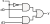
\includegraphics[scale=0.9]{img/circuito_mux1.pdf}}
    \end{center}
    \end{textblock}
    \begin{textblock}{55}(10,25)
    \begin{onlyenv}<2->
\begin{lstlisting}
module mux2(d0, d1, s, y);
    input d0;
    input d1;
    input s;
    output y;
    wire ns, y1, y2;

    not g1 (ns, s);
    and g2 (y1, d0, ns);
    and g2 (y2, d1, s);
    or  g4 (y, y1, y2);
endmodule
\end{lstlisting}
    \end{onlyenv}
    \end{textblock}
    \begin{textblock}{160}(0,75)
    \begin{center}
    \uncover<4->{\textcolor{naranjauca}{¿Cómo podemos construir un multiplexor de 2 bits de ancho?}}
    \end{center}
    \end{textblock}
\end{frame}

\begin{frame}[fragile,t]
    \frametitle{Ejemplo: Estilo \texttt{Behavioral}}
    Utilizando operaciones aritméticas, lógicas, asignaciones y cambios en el flujo de control, podemos modelar un comportamiento específico.
    \begin{textblock}{70}(75,24)
    \uncover<2->{En este caso utilizamos las operaciones lógicas \texttt{and}, \texttt{or} y \texttt{not}, para definir el comportamiento.}
    \end{textblock}
    \begin{textblock}{65}(75,35)
    \uncover<3->{
\includegraphics[scale=0.9]{img/circuito_mux1_expresion.pdf}}
    \end{textblock}
    \begin{textblock}{30}(125,42)
    \footnotesize
    \uncover<3->{\textcolor{verdeuca}{Si bien podemos\\ traducir el código\\ a compuertas de\\ forma directa,\\ \textbf{su representación\\ no es la misma.}}}
    \end{textblock}
    \begin{textblock}{160}(0,75)
    \begin{center}
    \uncover<4->{Entonces, \textcolor{naranjauca}{¿Cómo podemos construir un multiplexor de 2 bits de ancho?}}
    \end{center}
    \end{textblock}
    \begin{textblock}{58}(10,25)
    \begin{onlyenv}<2->
\begin{lstlisting}
module mux2(d0, d1, s, y);
    input d0;
    input d1;
    input s;
    output y;

    assing y = ~d0 &  d1 &  s 
              | d0 & ~d1 & ~s 
              | d0 &  d1 & ~s 
              | d0 &  d1 &  s;
endmodule
\end{lstlisting}
    \end{onlyenv}
    \end{textblock}
\end{frame}

\begin{frame}[fragile,t]
    \frametitle{Ejemplo: Estilo \texttt{Behavioral}}
    Para definir comportamientos más complejos tenemos el \texttt{if-then-else} \emph{inline}.
    \begin{textblock}{70}(80,20)
    \uncover<2->{Se asigna \texttt{d0} a la salida si \texttt{s} es $0$ y \texttt{d1} si \texttt{s} vale $1$.}\\
    \begin{center}
    \uncover<2->{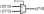
\includegraphics[scale=0.9]{img/mux1_8bits.pdf}}
    \end{center}
    \uncover<3->{\textcolor{verdeuca}{Como las entradas y salidas tiene ancho 8 bits, el circuito se comportará como un multiplexor de 2 entradas de 8 bits de ancho.}}\\
    \bigskip
    \uncover<5->{En este caso el operador de asignación condicional describe un comportamiento,\\ \textbf{no indica como este debe ser implementado}.}
    \end{textblock}
    \begin{textblock}{65}(10,20)
    \begin{onlyenv}<2->
\begin{lstlisting}
module mux2(d0, d1, s, y);
    input [7:0] d0, d1;
    input s;
    output [7:0] y;
    assign y = s ? d1 : d0;
endmodule
\end{lstlisting}
    \end{onlyenv}
    \begin{onlyenv}<4->
    Incluso se pueden anidar.
\begin{lstlisting}
module mux4(d0, d1, d2, d3, s, y);
    input [7:0] d0, d1, d2, d3;
    input s;
    output [7:0] y;
    assign y = s[1] ? 
                 (s[0] ? d1: d0) 
               : (s[0] ? d3: d2);
endmodule
\end{lstlisting}
    \end{onlyenv}
    \end{textblock}
\end{frame}

\begin{frame}[fragile,t]
    \frametitle{Ejemplo: Estilo \texttt{Behavioral}}
    \begin{textblock}{70}(80,10)
    \uncover<2->{
    O bien utilizando varios multiplexores en cascada.
    \begin{center}
    
\includegraphics[scale=0.9]{img/mux2_8bits.pdf}
    \end{center}
    }
    \uncover<3->{
    O bien utilizando un solo multiplexor de cuatro entradas.
    \begin{center}
    
\includegraphics[scale=0.9]{img/mux2_8bits_simple.pdf}
    \end{center}
    }
    \end{textblock}
    \begin{textblock}{65}(10,12)
    Al definir un comportamiento este puede implementarse de múltiples formas, dependiendo de las \textbf{celdas disponibles}.
    \bigskip
    \begin{onlyenv}<1->
\begin{lstlisting}
module mux4(d0, d1, d2, d3, s, y);
    input [7:0] d0, d1, d2, d3;
    input s;
    output [7:0] y;
    assign y = s[1] ?
                 (s[0] ? d1: d0) 
               : (s[0] ? d3: d2);
endmodule
\end{lstlisting}
    \end{onlyenv}
    \end{textblock}
\end{frame}

\begin{frame}[fragile,t]
    \frametitle{Ejemplo: Estilo \texttt{Behavioral}}
    Las operaciones pueden ser aplicadas sobre múltiples bits simultáneamente.\\
    Es decir, utilizarlos como buses de datos.
    \begin{textblock}{80}(10,25)
\begin{lstlisting}
    module gate(a, b, y1, y2, y3, y4, y5);
        input [3:0] a, b;
        output [3:0] y1, y2, y3, y4, y5;

        assign y1 = a & b;    // AND
        assign y2 = a | b;    // OR
        assign y3 = a ^ b;    // XOR
        assign y4 = ~(a & b); // NAND
        assign y5 = ~(a | b); // NOR

    endmodule
\end{lstlisting}
    \end{textblock}
    \begin{textblock}{60}(90,25) \begin{center} \uncover<1->{\includegraphics[scale=0.9]{img/circuito_ejemplo_operaciones-layer1.pdf}} \end{center} \end{textblock}
    \begin{textblock}{60}(90,25) \begin{center} \uncover<2->{\includegraphics[scale=0.9]{img/circuito_ejemplo_operaciones-layer2.pdf}} \end{center} \end{textblock}
\end{frame}

\begin{frame}[fragile,t]
    \frametitle{Ejemplo: Estilo \texttt{Behavioral}}
    Algunas de las operaciones se pueden usar como \textbf{operadores de reducción}.\\
    Estas actúan siempre sobre un conjunto de bits.
    \begin{textblock}{70}(10,23)
    \begin{onlyenv}<2->
\begin{lstlisting}
module and8(a, y);
    input [7:0] a;
    output y;

    assign y = &a;    
endmodule
\end{lstlisting}
    \end{onlyenv}
    \begin{onlyenv}<3->
    Equivalente a la siguiente sentencia,
\begin{lstlisting}
    ...
    assign y = a[7] & a[6] & a[5]
             & a[4] & a[3] & a[2]
             & a[1] & a[0];
    ...    
\end{lstlisting}
    \end{onlyenv}
    \end{textblock}
    \begin{textblock}{60}(85,25)
    \uncover<2->{
    En el ejemplo, el resultado en \textbf{\texttt{y}} es equivalente a realizar un \texttt{and} entre todos los bits de \textbf{\texttt{a}}.\\
    \bigskip
    \begin{center}
    
\includegraphics[scale=0.9]{img/circuito_and_x8.pdf}
    \end{center}
    }
    \end{textblock}
\end{frame}

\begin{frame}[fragile,t]
    \frametitle{Ejemplo: Buffer de tres estados}
    Este es uno de los circuitos más simples que podemos implementar utilizando el valor \texttt{z}.
    \begin{textblock}{70}(10,22)
    \begin{onlyenv}<2->
\begin{lstlisting}
module bufferTresEstados(a, en, y);
    input [3:0] a;
    input en;
    output [3:0] y;

    assign y = en ? a : 4'bzzzz;

endmodule
\end{lstlisting}
    \end{onlyenv}
    \uncover<2->{
    Si la señal \textbf{\texttt{en}} está en uno deja pasar la señal \textbf{\texttt{a}}, sino deja el circuito en alta impedancia (\emph{z}).\\
    \begin{center}
    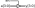
\includegraphics[scale=0.9]{img/buffer_3_estados.pdf}
    \end{center}
    }
    \end{textblock}
    \begin{textblock}{60}(86,22)
    \uncover<3->{
    Este comportamiento se utiliza para compartir un bus entre varias señales.\\
    \begin{center}
    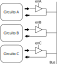
\includegraphics[scale=0.7]{img/bus_compartido.pdf}
    \end{center}
    }
    \end{textblock}
\end{frame}

\begin{frame}[fragile,t]
    \frametitle{Respuesta completa de compuertas}
    Las compuertas como entradas pueden recibir también los estados \texttt{Z} y \texttt{X}.    
    \begin{textblock}{60}(10,20)
    \begin{tabular}{|C{0.8cm}|c|c|c|c|} \hline
     \na \texttt{and} & \gm \texttt{0} & \gm \texttt{1} & \gm \texttt{x} & \gm \texttt{z} \\ \hline
     \gm \texttt{0}   & \texttt{0} & \texttt{0} & \texttt{0} & \texttt{0} \\ \hline 
     \gm \texttt{1}   & \texttt{0} & \texttt{1} & \texttt{x} & \texttt{x} \\ \hline 
     \gm \texttt{x}   & \texttt{0} & \texttt{x} & \texttt{x} & \texttt{x} \\ \hline 
     \gm \texttt{z}   & \texttt{0} & \texttt{x} & \texttt{x} & \texttt{x} \\ \hline 
    \end{tabular}
    \end{textblock}
    \begin{textblock}{60}(60,20)
    \begin{tabular}{|C{0.8cm}|c|c|c|c|} \hline
     \na \texttt{or}  & \gm \texttt{0} & \gm \texttt{1} & \gm \texttt{x} & \gm \texttt{z} \\ \hline
     \gm \texttt{0}   & \texttt{0} & \texttt{1} & \texttt{x} & \texttt{x} \\ \hline 
     \gm \texttt{1}   & \texttt{1} & \texttt{1} & \texttt{1} & \texttt{1} \\ \hline 
     \gm \texttt{x}   & \texttt{x} & \texttt{1} & \texttt{x} & \texttt{x} \\ \hline 
     \gm \texttt{z}   & \texttt{x} & \texttt{1} & \texttt{x} & \texttt{x} \\ \hline 
    \end{tabular}
    \end{textblock}
    \begin{textblock}{60}(110,20)
    \begin{tabular}{|C{0.8cm}|c|c|c|c|} \hline
     \na \texttt{xor} & \gm \texttt{0} & \gm \texttt{1} & \gm \texttt{x} & \gm \texttt{z} \\ \hline
     \gm \texttt{0}   & \texttt{0} & \texttt{1} & \texttt{x} & \texttt{x} \\ \hline 
     \gm \texttt{1}   & \texttt{1} & \texttt{0} & \texttt{x} & \texttt{x} \\ \hline 
     \gm \texttt{x}   & \texttt{x} & \texttt{x} & \texttt{x} & \texttt{x} \\ \hline 
     \gm \texttt{z}   & \texttt{x} & \texttt{x} & \texttt{x} & \texttt{x} \\ \hline 
    \end{tabular}
    \end{textblock}
    \begin{textblock}{60}(10,50)
    \begin{tabular}{|C{0.8cm}|c|c|c|c|} \hline
     \na \texttt{nand}& \gm \texttt{0} & \gm \texttt{1} & \gm \texttt{x} & \gm \texttt{z} \\ \hline
     \gm \texttt{0}   & \texttt{1} & \texttt{1} & \texttt{1} & \texttt{1} \\ \hline 
     \gm \texttt{1}   & \texttt{1} & \texttt{0} & \texttt{x} & \texttt{x} \\ \hline 
     \gm \texttt{x}   & \texttt{1} & \texttt{x} & \texttt{x} & \texttt{x} \\ \hline 
     \gm \texttt{z}   & \texttt{1} & \texttt{x} & \texttt{x} & \texttt{x} \\ \hline 
    \end{tabular}
    \end{textblock}
    \begin{textblock}{60}(60,50)
    \begin{tabular}{|C{0.8cm}|c|c|c|c|} \hline
     \na \texttt{nor} & \gm \texttt{0} & \gm \texttt{1} & \gm \texttt{x} & \gm \texttt{z} \\ \hline
     \gm \texttt{0}   & \texttt{1} & \texttt{0} & \texttt{x} & \texttt{x} \\ \hline 
     \gm \texttt{1}   & \texttt{0} & \texttt{0} & \texttt{0} & \texttt{0} \\ \hline 
     \gm \texttt{x}   & \texttt{x} & \texttt{0} & \texttt{x} & \texttt{x} \\ \hline 
     \gm \texttt{z}   & \texttt{x} & \texttt{0} & \texttt{x} & \texttt{x} \\ \hline 
    \end{tabular}
    \end{textblock}
    \begin{textblock}{60}(110,50)
    \begin{tabular}{|C{0.8cm}|c|c|c|c|} \hline
     \na \texttt{xnor}& \gm \texttt{0} & \gm \texttt{1} & \gm \texttt{x} & \gm \texttt{z} \\ \hline
     \gm \texttt{0}   & \texttt{1} & \texttt{0} & \texttt{x} & \texttt{x} \\ \hline 
     \gm \texttt{1}   & \texttt{0} & \texttt{1} & \texttt{x} & \texttt{x} \\ \hline 
     \gm \texttt{x}   & \texttt{x} & \texttt{x} & \texttt{x} & \texttt{x} \\ \hline 
     \gm \texttt{z}   & \texttt{x} & \texttt{x} & \texttt{x} & \texttt{x} \\ \hline 
    \end{tabular}
    \end{textblock}
\end{frame}

\begin{frame}[fragile,t]
    \frametitle{Módulos Parametrizados}
    \small
    Permite incluir variables dentro de módulos que pueden ser definidas al momento de la instanciación.\\
\begin{lstlisting}
    module mux2 #(parameter width = 8) (d0, d1, s, y);
        input  [width-1:0] d0, d1; input s;
        output [width-1:0] y;
        assign y = s ? d1 : d0;        
    endmodule
\end{lstlisting}
    \pause
    Si no se completa el parámetro, este toma su valor por defecto. Para el ejemplo 8.\\
\begin{lstlisting}
    mux2 i_mux_a(d0, d1, s, out);
\end{lstlisting}
    \pause
    Es posible instanciarlo indicando los argumentos de forma posicional.\\
\begin{lstlisting}
    mux2 #(12) i_mux_b(d0, d1, s, out);
\end{lstlisting}
    \pause
    O indicando el nombre de cada uno, incluyendo el parámetro.\\
\begin{lstlisting}
    mux2 #(.width(12)) i_mux_b(.d0(d0), .d1(d1), .s(s), .out(y));
\end{lstlisting}
\end{frame}

\begin{frame}[fragile,t]
    \frametitle{Circuitos Secuenciales}
    \begin{textblock}{70}(10,14)
    Para definir circuitos secuenciales necesitamos una nueva construcción del lenguaje \texttt{Verilog}.\\
    \end{textblock}
    \begin{textblock}{55}(90,12)
\begin{lstlisting}
always @ (sensitivity list)
    statement;
\end{lstlisting}
    \end{textblock}
    \begin{textblock}{140}(10,27)
    \uncover<2->{
    La sentencia \texttt{always} permite definir un \textbf{bloque de expresiones} que
    serán ``ejecutadas'' cada vez que alguna variable dentro de la \textbf{lista de sensibilidad}
    (\emph{sensitivity list}) sea modificada.\\
    }
    \bigskip
    \uncover<3->{
    La lista de sensibilidad debe contener una lista de variables y
    una indicación de tipo de cambio esperado. Este puede ser:
    \begin{itemize}
    \item \textcolor{naranjauca}{\texttt{posedge}}: Cambia en el flanco ascendente de reloj
    (Cambio de \texttt{0} a \texttt{1}).
    \item \textcolor{naranjauca}{\texttt{negedge}}: Cambia en el flanco descendente de reloj
    (Cambio de \texttt{1} a \texttt{0}).
    \end{itemize}
    }
    \vspace{0.2cm}
    \uncover<4->{
    \small
    \textcolor{verdeuca}{Se puede utilizar \texttt{*} para indicar que la sentencia es sensible a cualquier cambio,\\ o no indicar cambio y se toma por nivel.\\}
    \bigskip
    \textcolor{rojo}{\textbf{Importante} Incluir mal las variables implica un comportamiento final no esperado.\\}
    }
    \end{textblock}
\end{frame}

\begin{frame}[fragile,t]
    \frametitle{Ejemplo registro}
    \begin{textblock}{53}(10,15)
\begin{lstlisting}
module register(clk, d, q);
    input  clk;
    input  [3:0] d;
    output [3:0] q;
    reg [3:0] q;
    
    always @ (posedge clk)
    begin
        q <= d;
    end

endmodule
\end{lstlisting}
    \end{textblock}
    \begin{textblock}{80}(70,7)
    \uncover<2->{
    Las palabras reservadas \texttt{begin} y \texttt{end} indican donde comienza y termina el bloque \texttt{always}.\\
    \textcolor{verdeuca}{ {\small Si solo se tiene un \emph{statement} dentro del bloque se puede presindir de estas indicaciones.} }\\
    }
    \bigskip
    \uncover<3->{
    El valor de \texttt{q} solo se actualizará cuando el \texttt{clk} cambie de \texttt{0} a \texttt{1}.
    Entonces, el valor de \texttt{d} será copiado a \texttt{q}.\\
    }
    \bigskip
    \uncover<4->{
    Toda variable que será asignada o no dependiendo del tiempo, debe ser declarada como registro (\texttt{reg}).\\
    \textcolor{verdeuca}{El nombre \texttt{reg} no implica directamente una memoria.\\
    Dependiendo del contexto se puede materializar como memoria (\texttt{flip-flop}/\texttt{latch}) o
    como cables.}
    }
    \end{textblock}
    \begin{textblock}{150}(10,72)
    \uncover<5->{
    Dentro del bloque \texttt{always} no se permite usar \texttt{assign}.\\
    Se utilizan \emph{Non-Blocking assingment} {\Large (\textcolor{naranjauca}{\texttt{<=}})} y
    \emph{Blocking assingment} {\Large (\textcolor{naranjauca}{\texttt{=}})}
    }
    \end{textblock}
\end{frame}

\begin{frame}[fragile,t]
    \frametitle{Asignaciones Non-Blocking vs Blocking}
    \begin{textblock}{40}(10,15)
    \begin{onlyenv}<1->
    \textbf{NonBlocking} {\Large (\textcolor{naranjauca}{\texttt{<=}})}
\begin{lstlisting}
    always @ (a)
    begin
        a <= 2'b01;
        b <= a;
    end
\end{lstlisting}
    \end{onlyenv}
    \end{textblock}
    \begin{textblock}{90}(52,15)
    \begin{itemize}
     \item<1-> Todas las asignaciones se hacen al final del bloque, \textbf{todas al mismo tiempo}.
     \item<2-> Se realizan \textbf{en paralelo}, con los valores que YA tenían las variables que son usadas del lado derecho.
     \item<3-> \textcolor{verdeuca}{En el ejemplo \texttt{b} toma el valor que a tenia en el pasado y no \texttt{2'b01}}
    \end{itemize}
    \end{textblock}

    \begin{textblock}{40}(10,52)
    \begin{onlyenv}<4->
    \textbf{Blocking} {\Large (\textcolor{naranjauca}{\texttt{=}})}
\begin{lstlisting}
    always @ (a)
    begin
        a = 2'b01;
        b = a;
    end
\end{lstlisting}
    \end{onlyenv}
    \end{textblock}
    \begin{textblock}{90}(52,52)
    \begin{itemize}
    \item<4-> Cada asignación es ejecutada \textbf{inmediatamente}.
    \item<5-> Se ejecutan en orden, es similar a la \textbf{ejecución secuencial}. Hasta que no se termina de ejecutar la asignación anterior, no se continua con la siguiente.
    \item<6-> \textcolor{verdeuca}{En el ejemplo \texttt{b} toma el valor \texttt{2'b01}}
    \end{itemize}
    \end{textblock}
\end{frame}

\begin{frame}[fragile,t]
    \frametitle{Ejemplos de asignaciones bloqueantes y no bloqueantes}
    \begin{textblock}{40}(10,15)
    \begin{onlyenv}<1->
\begin{lstlisting}
    always @ (*)
    begin
        p <= a & b;
        q <= a ~^ b;
        r <= p | q;
    end
\end{lstlisting}
    \end{onlyenv}
    \end{textblock}
    \begin{textblock}{90}(60,15)
    \uncover<1->{\textbf{NonBlocking} {\Large (\textcolor{naranjauca}{\texttt{<=}})}}\\
    \uncover<2->{Suponer \texttt{a=0}, \texttt{b=1}. Tanto \texttt{p}, \texttt{q} y \texttt{r} valen cero.}
    \uncover<3->{Si cambia \texttt{b} a \texttt{0}.}\\
    \uncover<4->{Entonces \texttt{p} será \texttt{0}, \texttt{q} será \texttt{1},}
    \uncover<5->{\textcolor{verdeuca}{\textbf{pero \texttt{r} utilizará los valores anteriores de \texttt{p} y \texttt{q}, resultando en cero.}}}\\
    \uncover<6->{$\rightarrow$ \textcolor{naranjauca}{Se asigna en paralelo}.}
    \end{textblock}
    \begin{textblock}{40}(10,50)
    \begin{onlyenv}<7->
\begin{lstlisting}
    always @ (*)
    begin
        p = a & b;
        q = a ~^ b;
        r = p | q;
    end
\end{lstlisting}
    \end{onlyenv}
    \end{textblock}
    \begin{textblock}{90}(60,50)
    \uncover<7->{\textbf{Blocking} {\Large (\textcolor{naranjauca}{\texttt{=}})}}\\
    \uncover<8->{Suponer \texttt{a=0}, \texttt{b=1}. Tanto \texttt{p}, \texttt{q} y \texttt{r} valen cero.}
    \uncover<9->{Si cambia \texttt{b} a \texttt{0}.}\\
    \uncover<10->{Entonces \texttt{p} será \texttt{0}, \texttt{q} será \texttt{1}.}
    \uncover<11->{\textcolor{verdeuca}{\textbf{\texttt{r} tomará los nuevos valores\\ de \texttt{p} y \texttt{q}, resultando en uno.}}}\\
    \uncover<12->{$\rightarrow$ \textcolor{naranjauca}{Se asigna secuencialmente}.}
    \end{textblock}
\end{frame}

\begin{frame}[fragile,t]
    \frametitle{Reglas de asignación de señales}
    \small
    \only<1->{Usar \textcolor{verdeuca}{\texttt{always @(posedge clk)}} y asignaciones no bloqueantes (\texttt{<=}), implica modelar lógica secuencial.\\}
    \only<1->{\hspace{1cm} \textcolor{gray}{Ejemplo:} \hspace{0.5cm} \textcolor{gray}{\texttt{always @ (posedge clk) q <= d;}}\\}
    \bigskip
    \only<2->{Usar asignaciones (\textcolor{verdeuca}{\texttt{assign}}), implica modelar lógica combinacional.\\}
    \only<2->{\hspace{1cm} \textcolor{gray}{Ejemplo:} \hspace{0.5cm} \textcolor{gray}{\texttt{assign y = a \& b;}}\\}
    \bigskip
    \only<3->{Usar \textcolor{verdeuca}{\texttt{always @(*)}} y asignaciones bloqueantes (\texttt{=}), implica modelar lógica combinatoria más compleja.\\}
    \vspace{1cm}
    \only<4->{Además no es posible hacer asignaciones a la misma señal desde múltiples bloques \texttt{always} o simultáneamente en un \texttt{assign}.\\}
    \only<4->{\hspace{1cm} \textcolor{gray}{Ejemplo:\\ \hspace{0.6cm} (No se puede)}}
    \begin{textblock}{30}(40,63)
    \begin{onlyenv}<4->
\lstset{moredelim=[is][\sout]{|}{|}, backgroundcolor=\color{rojo!20}}
\begin{lstlisting}
|always @(*)|
    |a = b;|
|always @(*)|
    |a = c;|
\end{lstlisting}
    \end{onlyenv}
    \end{textblock}
    \begin{textblock}{30}(80,63)
    \begin{onlyenv}<4->
\lstset{moredelim=[is][\sout]{|}{|}, backgroundcolor=\color{rojo!20}}
\begin{lstlisting}
|always @(*)|
    |a = b;|
|assign a = c;|
\end{lstlisting}
    \end{onlyenv}
    \end{textblock}
\end{frame}

\begin{frame}[fragile,t]
    \frametitle{Sentencia \texttt{if}}
    \begin{textblock}{65}(10,16)
    La sentencia \texttt{if} es ejecutada de\\ \textbf{forma paralela}.\\
    \bigskip
    \uncover<2->{Se debe pensar como que describe simultáneamente dos flujos diferentes y que ambos se ejecutan todo el tiempo.}\\
    \bigskip
    \uncover<3->{\textcolor{verdeuca}{Para utilizar más de una sentencia dentro de \texttt{if/else} se pueden usar las palabras reservas \texttt{begin} y \texttt{end} para agrupar el conjunto de sentencias.}}
    \end{textblock}
    \begin{textblock}{70}(80,12)
    \textcolor{gray}{Ejemplo:}\\
\begin{lstlisting}
module abs(data, result);
    input [7:0] data;
    output [7:0] result;
    reg [7:0] result;

    always @ (*)
      if (result[7])
        result <= {1'b0, data[6:0]};
      else
        result <= data;
endmodule
\end{lstlisting}
    \end{textblock}
\end{frame}

\begin{frame}[fragile,t]
    \frametitle{Sentencia \texttt{case}}
    \begin{textblock}{60}(10,15)
    La sentencia \texttt{case} permite decidir entre un conjunto de posibilidades.\\
    \bigskip
    \uncover<2->{\textcolor{verdeuca}{Su implementación es equivalente a una serie de \texttt{if} anidados uno detras del otro.}}\\
    \bigskip
    \uncover<3->{Existen además las sentencias \texttt{casez} y \texttt{casex} que permiten incluir valores en las etiquetas valores no definidos.}
    \end{textblock}
    \begin{textblock}{65}(80,5)
    \textcolor{gray}{Ejemplo:}\\
\begin{lstlisting}
module GraySeq(seq, gray);
    input [3:0] seq;
    output [3:0] gray;
    reg [3:0] gray;
    always @ (*)
    begin
        case (seq)
        4'd0:    gray = 4'b0000;
        4'd1:    gray = 4'b0001;
        4'd2:    gray = 4'b0011;
        4'd3:    gray = 4'b0010;
        4'd4:    gray = 4'b0110;
        4'd5:    gray = 4'b0111;
        4'd6:    gray = 4'b0101;
        4'd7:    gray = 4'b0100;
        default: gray = 4'b0000;
        endcase
    end
endmodule
\end{lstlisting}
    \end{textblock}
\end{frame}

\begin{frame}[fragile,t]
    \frametitle{Sentencia \texttt{casez} y \texttt{casex}}
    \begin{textblock}{64}(10,12.3)
    \textcolor{gray}{Ejemplo:} \texttt{casez}\\
\lstset{basicstyle=\scriptsize}
\begin{lstlisting}
module deco(opcode, command);
    input [4:0] opcode;
    output [2:0] command;
    reg [2:0] command;
    always @ (*)
    begin
        casez (opcode)
        4'b0???1: command = 1;
        4'b0??10: command = 2;
        4'b0?100: command = 3;
        4'b01000: command = 4;
        4'b11000: command = 5;
        default:  command = 7;
        endcase
    end
endmodule
\end{lstlisting}
    \small
    \textcolor{naranjauca}{\texttt{\textbf{casez:}}} No considera como parte de la comparación los bits marcados como \texttt{?} o \texttt{z}.
    \end{textblock}
    \begin{textblock}{64}(85,9)
    \textcolor{gray}{Ejemplo:} \texttt{casex}\\
\lstset{basicstyle=\scriptsize}
\begin{lstlisting}
module PriorityEncoder(sel, bit);
    input [5:0] sel;
    output [2:0] bit;
    reg [2:0] bit;
    always @ (*)
    begin
        casex (sel)
        6'bxxxxx1: bit = 1;
        6'bxxxx1x: bit = 2;
        6'bxxx1xx: bit = 3;
        6'bxx1xxx: bit = 4;
        6'bx1xxxx: bit = 5;
        6'b1xxxxx: bit = 6;
        default:   bit = 0;
        endcase
    end
endmodule
\end{lstlisting}
    \small
    \textcolor{naranjauca}{\texttt{\textbf{casex:}}} No considera como parte de la comparación los bits marcados como \texttt{?} o \texttt{z} o \texttt{x}.
    \end{textblock}
\end{frame}

\begin{frame}[fragile,t]
    \frametitle{Señales sincrónicas y asincrónicas}
    Los circuitos reciben señales que respetan alguna semántica temporal.
    \begin{itemize}
    \item<2-> \textbf{Señales Sincrónicas}\\
    Dependen del reloj, se leen en un momento preciso del tiempo.
    \item<3-> \textbf{Señales Asincrónicas}\\
    Se pueden dar en cualquier momento y afectan al circuito instantáneamente.
    \end{itemize}
    \bigskip
    \uncover<4->{\textbf{\textcolor{naranjauca}{Señal de \texttt{reset}}}}\\
    \uncover<4->{Se utiliza para inicializar el hardware. Setea los circuitos a un estado conocido, o de inicio.}\\
    \begin{itemize}
    \item<5-> \textbf{Reset Asincrónico}: Independiente del clock.\\
    Actuá con máxima prioridad (antes que todo).\\
    \textcolor{verdeuca}{Es sensible a \emph{glitches} que pueden generar problemas de estabilidad del circuito.}
    \item<6-> \textbf{Reset Sincrónico}: Respeta los cambios del clock.\\
    La activación se debe prolongar por el tiempo necesario para el cambio de clock.\\
    \textcolor{verdeuca}{El resultado es sincrónico con el circuito, no genera problemas de estabilidad.}
    \end{itemize}
\end{frame}
   
\begin{frame}[fragile,t]
    \frametitle{Ejemplo: Reset asincrónico}
    \begin{textblock}{75}(10,15)
\begin{lstlisting}
module register_AR(clk, reset, d, q);
  input  clk;
  input  reset;
  input  [3:0] d;
  output [3:0] q;
  reg [3:0] q;
    
  always @ (posedge clk, negedge reset)
  begin
      if (reset == 1)
          q <= 0;
      else
          q <= d;
  end
endmodule
\end{lstlisting}
    \end{textblock}
    \begin{textblock}{60}(90,15)
    \uncover<1->{El reset se chequea al comienzo del bloque, si es \texttt{1} entonces se setea \texttt{q} a \texttt{0}.}\\
    \bigskip
    \uncover<2->{La lista de sensibilidad incluye el cambio de la señal de reset a cero.}\\
    \bigskip
    \uncover<3->{\textcolor{gray}{Es un reset asincronico, porque el cambio puede suceder independiente al cambio del reloj.}}
    \end{textblock}
\end{frame}

\begin{frame}[fragile,t]
    \frametitle{Ejemplo: Reset sincrónico}
    \begin{textblock}{75}(10,15)
\begin{lstlisting}
module register_SR(clk, reset, d, q);
  input  clk;
  input  reset;
  input  [3:0] d;
  output [3:0] q;
  reg [3:0] q;
    
  always @ (posedge clk)
  begin
      if (reset == 1)
          q <= 0;
      else
          q <= d;
  end
endmodule
\end{lstlisting}
    \end{textblock}
    \begin{textblock}{60}(90,15)    
    \uncover<1->{El reset se chequea al comienzo del bloque, si es \texttt{1} entonces se setea \texttt{q} a \texttt{0}.}\\
    \bigskip
    \uncover<2->{La lista de sensibilidad \textbf{solo} incluye al reloj. Por lo tanto solo va a actuar si se altera el reloj.}\\
    \bigskip
    \uncover<3->{\textcolor{gray}{Es un reset sincronico, porque el cambio por la señal de reset solo puede actuar ante un cambio en la señal de reloj.}}
    \end{textblock}
\end{frame}

\begin{frame}[fragile,t]
    \frametitle{Ejemplo: Enable sincrónico y reset asincrónico}
    \begin{textblock}{75}(10,15)
\begin{lstlisting}
module reg_SR(clk, reset, en, d, q);
  input  clk;
  input  reset;
  input  en;
  input  [3:0] d;
  output [3:0] q;
  reg [3:0] q;
    
  always @ (posedge clk, negedge reset)
  begin
      if (reset == 1)
          q <= 0;
      else
          if (en)
              q <= d;
  end
endmodule
\end{lstlisting}
    \end{textblock}
    \begin{textblock}{63}(90,15)
    \uncover<1->{El registro tiene dos señales adicionales \emph{enable} y \emph{reset}.}\\
    \bigskip
    \uncover<2->{Notar que la señal de \textbf{\emph{enable} no figura en la lista de sensibilidad}.}\\
    \bigskip
    \uncover<3->{El comportamiento respeta que \texttt{q} toma el valor de \texttt{d}, solo cuando hay un flanco ascendente del reloj y el \texttt{enable} está en \texttt{1}.}
    \end{textblock}
\end{frame}

\begin{frame}[fragile,t]
    \frametitle{Ejemplo: Latch}
    \begin{textblock}{60}(10,15)
\begin{lstlisting}
module latch(clk, d, q);
    input  clk;
    input  [3:0] d;
    output [3:0] q;
    reg [3:0] q;
    
    always @ (clk, d)
        if (clk) q <= d;
        
endmodule
\end{lstlisting}
    \end{textblock}
    \begin{textblock}{65}(80,15)
    \uncover<1->{El \emph{latch}, a diferencia de un registro, funciona con el valor de nivel del reloj.}\\
    \bigskip
    \uncover<2->{Si el nivel es alto toma el valor, si el nivel es bajo no toma el valor.}\\
    \bigskip
    \uncover<3->{\textcolor{verdeuca}{Con dos latch se puede construir un flip-flop activado por flanco, como \emph{master-slave}.}}
    \end{textblock}
\end{frame}

\begin{frame}[fragile,t]
    \frametitle{Lógica combinacional vs lógica secuencial}
    \begin{textblock}{65}(10,10)
    \begin{onlyenv}<1->
\begin{lstlisting}
module seq(clk, d, q);
    input  clk; input  [3:0] d;
    output [3:0] q;
    reg [3:0] q;
    always @ (posedge clk)
        q <= d;
endmodule
\end{lstlisting}
    \end{onlyenv}
    \small
    \uncover<1->{El bloque \emph{always} describe la señal \texttt{q}.}\\
    \vspace{0.2cm}
    \uncover<2->{Esta solo se modifica cuando hay un flanco ascendente de reloj.}\\
    \vspace{0.2cm}
    \uncover<3->{Durante el resto del tiempo el circuito expone el valor anterior.}\\
    \vspace{0.2cm}
    \uncover<4->{\textcolor{verdeuca}{El resultado es un circuito secuencial, genera una memoria, porque \textbf{recuerda}.}}
    \end{textblock}
    \begin{textblock}{65}(85,10)
    \begin{onlyenv}<5->
\begin{lstlisting}
module comb(inv data, result);
    input  inv; input  [3:0] data;
    output [3:0] result;
    reg [3:0] result;
    always @ (inv, data)
        if (inv)
            result <= ~data;
        else
            result <= data;
endmodule
\end{lstlisting}
    \end{onlyenv}
    \small
    \uncover<6->{Si \texttt{inv} vale \texttt{1}, expone en \texttt{result} el valor de \texttt{data} negado bit a bit.}
    \uncover<6->{Si \texttt{inv} vale \texttt{0}, no invierte.}\\
    \vspace{0.2cm}
    \uncover<7->{Cualquier cambio de \texttt{inv} o de \texttt{data} va a cambiar \texttt{result}, no importa que cambie.}\\
    \vspace{0.2cm}
    \uncover<8->{El resultado es un circuito combinacional, no genera memoria, porque \textbf{siempre cambia}.}
    \end{textblock}
\end{frame}

\begin{frame}[fragile,t]
    \frametitle{Bloque \texttt{always} para circuitos combinatorios}
    Si bien el bloque \texttt{always} nos permite generar circuitos secuenciales,\\
    \textcolor{verdeuca}{el resultado de la sintesis será un \textbf{ciruito combinatorio} si:}\\
    \bigskip
    \begin{itemize}
    \setlength\itemsep{0.5cm}
    \item<2-> Todas las señales asignadas en el bloque son \textbf{siempre asignadas},\\
    en todos los caminos tenemos un valor para la señal (\emph{continuously assignment}).
    \item<3-> Todas las señales del lado derecho \textbf{pertenecen a la lista de sensibilidad}.\\
    Se puede usar \texttt{always @*} para implicar a todas las señales.
    \item<4-> Todas las señales en el lado izquierdo \textbf{son asignadas para cualquier caso} dentro de todos los bloques.
    Ojo con asignar parcialmente un bus de señales por error.
    \end{itemize}
    \bigskip
    \uncover<5->{\textcolor{red}{\textbf{Warning}: Es muy facil comenter errores y generar memorias (latch) no intencionales.}}
\end{frame}

\begin{frame}[fragile,t]
    \frametitle{Bloque \texttt{always} para circuitos combinatorios}
    \textcolor{gray}{Ejemplo:} \textcolor{red}{Errores en bloques \texttt{always} para construir circuitos combinatorios}
    \begin{textblock}{60}(10,18)
    \begin{onlyenv}<2->
    \lstset{basicstyle=\scriptsize}
\begin{lstlisting}
    ...
    wire enable, data;
    reg a, b;
    always @ (*)
    begin
        a = 0;
        
        if(enable)
        begin
            a = ~data;
            b = data;
        end
    end
    ...
\end{lstlisting}
    \textcolor{red}{Error}\\ \texttt{b} no está siendo asignado para cuando \texttt{enable} es \texttt{false}.
    \end{onlyenv}
    \end{textblock}
    \begin{textblock}{60}(85,18)
    \begin{onlyenv}<3->
    \lstset{basicstyle=\scriptsize}
\begin{lstlisting}
    ...
    wire enable, data;
    reg a, b;
    always @ (data)
    begin
        a = 1;
        b = 0;
        if(enable)
        begin
            a = ~data;
            b = data;
        end
    end
    ...
\end{lstlisting}
    \textcolor{red}{Error}\\ \texttt{enable} no esta en la lista de sensibilidad.
    \end{onlyenv}
    \end{textblock}
\end{frame}

\begin{frame}[fragile,t]
    \frametitle{Bloque \texttt{always}: No siempre es práctico}
    Para cualquier operatoria que requiera código simple de condiciones y asignaciones, donde siempre se asignan datos.
    \textcolor{verdeuca}{Lo ideal es utilizar asignaciones.}
    \begin{textblock}{60}(10,24)
    \begin{onlyenv}<2->
    Opción 1
\begin{lstlisting}
    ...
    reg  [31:0] result;
    wire [31:0] a, b, comb;
    wire sel;

    always @ (a, b, sel)
    begin
        if (sel)
            result <= a;
        else
            result <= b;
    end
    ...
\end{lstlisting}
    \end{onlyenv}
    \end{textblock}
    \begin{textblock}{60}(85,24)
    \begin{onlyenv}<3->
    Opción 2
\begin{lstlisting}
    ...
    reg  [31:0] result;
    wire [31:0] a, b, comb;
    wire sel;

    assign comb = sel? a : b;
    ...
\end{lstlisting}
    \end{onlyenv}
    \end{textblock}
    \begin{textblock}{60}(85,65)
    \uncover<4->{\textcolor{naranjauca}{La opción 2 es más simple y no expone errores de creación de memorias no deseadas.}}
    \end{textblock}
\end{frame}

\begin{frame}[fragile,t]
    \frametitle{Definición de tiempos \emph{(Timing relations)}}
    \begin{itemize}
     \item<1-> Podemos simular tiempos pero no son objetivo para la sintetización.
     \item<2-> No podemos hacer que la sintetización reproduzca los tiempos indicados.\\
     La temporización está \textbf{definida por las celdas} que tengamos en el hardware.
     \item<3-> Los tiempos definidos se usan como \textbf{retardos dentro de la simulación}.
    \end{itemize}
    \begin{onlyenv}<4->
\begin{lstlisting}
    timescale 1ns/1ps
    module simple(input a, output z1, z2);
        assign #5 z1 = ~a;
        assign #9 z2 = a;
    endmodule
\end{lstlisting}
    \end{onlyenv}
    \small
    \uncover<4->{En el ejemplo:}
    \begin{itemize}
     \item<4-> \texttt{timescale 1ns/1ps}\\
     \textcolor{verdeuca}{Definimos la escala de tiempo para la simulación.}
     \item<4-> \verb|#5 z1 = ˜a;|\\
     \textcolor{verdeuca}{La asignación de \texttt{z1} será resuelta en \texttt{5} unidades de tiempo.}
    \end{itemize}
\end{frame}

\begin{frame}[fragile,t]
    \frametitle{Buenas practicas}
    A diferencia de escribir código en lenguajes de programación.\\
    En los HDL \textbf{debemos} ser muy ordenados y eficientes en el código.\\
    \textcolor{verdeuca}{Para esto hay un conjunto de reglas que ayudan en la tarea.\\}
    \bigskip
    \pause
    \textcolor{naranjauca}{\textbf{Usar un estilo de nombres consistente}}\\
    Los nombres de señales, entradas salidas y de cables deben ser claros,
    evitando ambigüedades, y reduciendo la posibilidad de confusiones.\\
    \bigskip
    \pause
    \textcolor{naranjauca}{\textbf{Orden de los bits}}\\
    Si bien es posible utilizar cualquier orden para los bits en un bus se recomienda:\\
    \texttt{a[31:0]}: Para cualquier número o bus de datos.\\
    \texttt{a[0:31]}: Solo para arreglos.\\
    \bigskip 
    \pause
    \textcolor{naranjauca}{\textbf{Diseño jerarquico}}\\
    Cada archivo debe tener un modulo particular, o conjunto de módulos relacionados.\\
    Respetar que el nombre del archivo siga una convención con el nombre del modulo.
\end{frame}

\begin{frame}[fragile]
    \frametitle{Bibliografía}
    \begin{itemize}
    \setlength\itemsep{0.5cm}
    \item[-] \textbf{``Digital Design and Computer Architecture''}, Second Edition\\
    David Money Harris, Sarah L. Harris - Morgan Kaufmann - 2013\\    
        \begin{itemize}
        \item Chapter 4 - Hardware Description Languages $\rightarrow$ Pag. 173-220
        \end{itemize}
    \item[-] \textbf{``Diseño Digital''}, Tercera Edicion\\
    M. Morris Mano - Pearson - 2003\\
        \begin{itemize}
        \item Capitulo 4-11 HDL para circuitos combinacionales $\rightarrow$ Pag. 147-160
        \item Capitulo 5-5 HDL para circuitos secuenciales $\rightarrow$ Pag. 190-197
        \end{itemize}
    \item[-] \textbf{``Digital Design and Verilog HDL Fundamentals''}\\
    Joseph Cavanagh - CRC Press, Taylor \& Francis Group - 2008\\
        \begin{itemize}
        \item Chapter 4 - Combinational Logic Design Using Verilog $\rightarrow$ Pag. 231-412
        \end{itemize}
    \end{itemize}
\end{frame}

\begin{frame}[plain]
    \begin{center}
    \vspace{2cm}
    \huge ¡Gracias!\\
    \vspace{2cm}
    \end{center}
\end{frame}

\end{document}

